
% header %{{{1

\documentclass[tikz, border=1mm]{standalone}

\usepackage{amsmath}
\usepackage{tikz}

\usetikzlibrary{calc,angles,quotes}

\tikzset{
	% ---- default
	every path/.style={line width=0.3pt},
	every coordinate/.style={fill=black, circle, inner sep=1pt},
	every node/.style={font=\normalsize},
	every picture/.style={scale=1.0},
	% ---- custom
	construction/.style={line width=0.1pt, dashed},
	dimension/.style={line width=0.2pt, <->, goldenbrown},
	dimension extension/.style={line width=0.2pt, dashed, goldenbrown},
	vector/.style={->, thick},
}

% document %{{{1

% opening %{{{2

\begin{document}

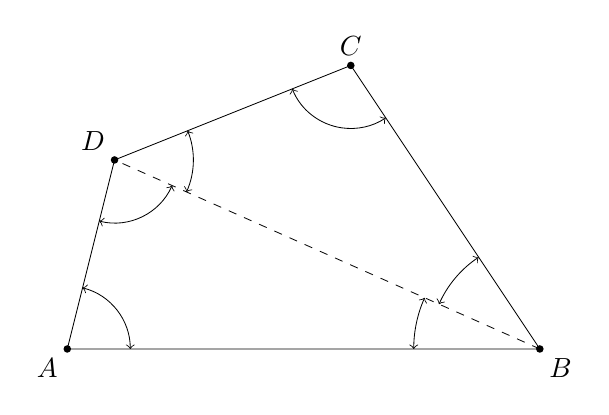
\begin{tikzpicture}[scale=1.2]

% coordinates %{{{2

	\coordinate (A) at (0,0);
	\coordinate (B) at (5,0);
	\coordinate (C) at (3,3);
	\coordinate (D) at (0.5,2);

% quadrilatere %{{{2

	\draw (A) -- (B) -- (C) -- (D) -- cycle;

% triangles %{{{2

	\draw[dashed] (B) -- (D);

% points, dots, vertices %{{{2

	\fill (A) circle (0.4mm);
	\fill (B) circle (0.4mm);
	\fill (C) circle (0.4mm);
	\fill (D) circle (0.4mm);

% points, dots, vertices labels %{{{2

	\node[below left] at (A) {$A$};
	\node[below right] at (B) {$B$};
	\node[above] at (C) {$C$};
	\node[above left] at (D) {$D$};

% angles labels %{{{2

	\pic[draw, <->, angle radius=0.8cm, angle eccentricity=1.0]
	{angle = B--A--D};

	\pic[draw, <->, angle radius=1.6cm, angle eccentricity=1.0]
	{angle = D--B--A};

	\pic[draw, <->, angle radius=1.4cm, angle eccentricity=1.0]
	{angle = C--B--D};

	\pic[draw, <->, angle radius=0.8cm, angle eccentricity=1.0]
	{angle = D--C--B};

	\pic[draw, <->, angle radius=1.0cm, angle eccentricity=1.0]
	{angle = B--D--C};

	\pic[draw, <->, angle radius=0.8cm, angle eccentricity=1.0]
	{angle = A--D--B};

% closing %{{{2

\end{tikzpicture}
\end{document}
